\documentclass[12pt, a4paper]{article}

% ── Packages ──────────────────────────────────────────────────────────────────
\usepackage{amsmath, amssymb, amsthm}
\usepackage{geometry}
\usepackage{booktabs}
\usepackage{array}
\usepackage{hyperref}
\usepackage{xcolor}
\usepackage{tcolorbox}
\usepackage{enumitem}
\usepackage{parskip}
\usepackage{tikz}
\usetikzlibrary{arrows.meta, positioning, calc}

\geometry{margin=2.5cm}

% ══════════════════════════════════════════════════════════════════════════════
% ── Student-mode switch ───────────────────────────────────────────────────────
\newif\ifstudentmode
\studentmodefalse

\ifx\studentflag\undefined
\else
  \studentmodetrue
\fi
% ══════════════════════════════════════════════════════════════════════════════

% ── Student-mode macros ───────────────────────────────────────────────────────
\newcommand{\sol}[2][6cm]{%
  \ifstudentmode
    \underline{\hspace{#1}}%
  \else
    {#2}%
  \fi
}

\newcommand{\soleq}[2][3cm]{%
  \ifstudentmode
    \par\vspace{4pt}%
    \noindent\rule{\linewidth}{0.5pt}\\[#1]%
    \noindent\rule{\linewidth}{0.5pt}%
    \par\vspace{4pt}%
  \else
    \[#2\]%
  \fi
}
% ──────────────────────────────────────────────────────────────────────────────

% ── Colors & boxes ────────────────────────────────────────────────────────────
\definecolor{mainblue}{RGB}{30, 100, 180}
\definecolor{boxbg}{RGB}{235, 243, 255}
\definecolor{notebg}{RGB}{255, 248, 230}
\definecolor{warnbg}{RGB}{255, 235, 235}
\definecolor{greenbg}{RGB}{230, 255, 235}

\tcbuselibrary{skins, breakable}

\newtcolorbox{resultbox}{
  colback=boxbg, colframe=mainblue,
  boxrule=1.2pt, arc=4pt,
  title={Result},
  fonttitle=\bfseries\color{white},
  coltitle=white, attach boxed title to top left={yshift=-2mm, xshift=4mm},
  boxed title style={colback=mainblue, arc=3pt}
}

\newtcolorbox{notebox}{
  colback=notebg, colframe=orange!70!black,
  boxrule=1pt, arc=4pt,
  left=4pt, right=4pt
}

\newtcolorbox{warnbox}{
  colback=warnbg, colframe=red!60!black,
  boxrule=1pt, arc=4pt,
  left=4pt, right=4pt
}

\newtcolorbox{stepbox}[1]{
  colback=greenbg, colframe=green!50!black,
  boxrule=1pt, arc=4pt,
  title={#1},
  fonttitle=\bfseries,
  coltitle=green!30!black
}
% ──────────────────────────────────────────────────────────────────────────────

% ── Theorem environments ───────────────────────────────────────────────────────
\theoremstyle{definition}
\newtheorem{example}{Example}[section]

% ── Math macros ───────────────────────────────────────────────────────────────
\newcommand{\yhat}{\hat{y}}
\newcommand{\sigmoid}{\sigma}
\newcommand{\bx}{\mathbf{x}}
\newcommand{\bh}{\mathbf{h}}
\newcommand{\bz}{\mathbf{z}}
\newcommand{\bW}{\mathbf{W}}
\newcommand{\bb}{\mathbf{b}}

% ── Document ──────────────────────────────────────────────────────────────────
\begin{document}

\begin{center}
  {\LARGE \textbf{Section 3.3: The Forward Pass}} \\[0.3em]
  {\large\itshape Computing a Prediction Step by Step} \\[0.5em]
  {\large AI Class --- Lecture Notes}%
  \ifstudentmode
    \quad {\normalsize\color{gray}[Student Copy]}%
  \fi
\end{center}

\vspace{1em}
\hrule
\vspace{1.5em}

% ══════════════════════════════════════════════════════════════════════════════
\section{The Network Architecture}

We will work with a \textbf{two-layer feedforward network} (one hidden layer)
designed to solve XOR:

\begin{center}
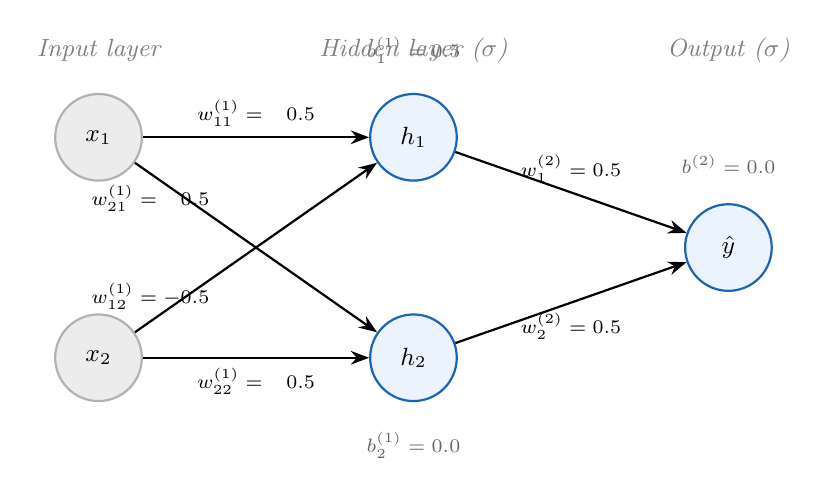
\begin{tikzpicture}[
  neuron/.style={circle, draw=mainblue, fill=boxbg,
                 minimum size=1.1cm, thick, font=\small},
  input/.style={circle, draw=gray!60, fill=gray!15,
                minimum size=1.1cm, thick, font=\small},
  >=Stealth, node distance=0pt
]
  % ── Nodes ──────────────────────────────────────────────────────────────────
  \node[input]   (x1) at (0,  1.4) {$x_1$};
  \node[input]   (x2) at (0, -1.4) {$x_2$};

  \node[neuron]  (h1) at (4,  1.4) {$h_1$};
  \node[neuron]  (h2) at (4, -1.4) {$h_2$};

  \node[neuron]  (yh) at (8,  0)   {$\yhat$};

  % ── Connections: input → hidden ────────────────────────────────────────────
  \draw[->, thick] (x1) -- node[above, font=\scriptsize, pos=0.5]
    {$w^{(1)}_{11}=\phantom{-}0.5$} (h1);
  \draw[->, thick] (x1) -- node[above left, font=\scriptsize, pos=0.35]
    {$w^{(1)}_{21}=\phantom{-}0.5$} (h2);
  \draw[->, thick] (x2) -- node[below left, font=\scriptsize, pos=0.35]
    {$w^{(1)}_{12}=-0.5$} (h1);
  \draw[->, thick] (x2) -- node[below, font=\scriptsize, pos=0.5]
    {$w^{(1)}_{22}=\phantom{-}0.5$} (h2);

  % ── Connections: hidden → output ───────────────────────────────────────────
  \draw[->, thick] (h1) -- node[above, font=\scriptsize, pos=0.5]
    {$w^{(2)}_1=0.5$} (yh);
  \draw[->, thick] (h2) -- node[below, font=\scriptsize, pos=0.5]
    {$w^{(2)}_2=0.5$} (yh);

  % ── Bias annotations ───────────────────────────────────────────────────────
  \node[font=\scriptsize, gray!80!black, above=0.25cm of h1]
    {$b^{(1)}_1 = 0.5$};
  \node[font=\scriptsize, gray!80!black, below=0.25cm of h2]
    {$b^{(1)}_2 = 0.0$};
  \node[font=\scriptsize, gray!80!black, above=0.25cm of yh]
    {$b^{(2)} = 0.0$};

  % ── Layer labels ───────────────────────────────────────────────────────────
  \node[font=\small\itshape, gray] at (0,  2.5) {Input layer};
  \node[font=\small\itshape, gray] at (4,  2.5) {Hidden layer ($\sigmoid$)};
  \node[font=\small\itshape, gray] at (8,  2.5) {Output ($\sigmoid$)};
\end{tikzpicture}
\end{center}

\vspace{0.5em}

The network has the following parameters:
\[
  \bW^{(1)} = \begin{bmatrix} 0.5 & -0.5 \\ 0.5 & \phantom{-}0.5 \end{bmatrix},
  \quad
  \bb^{(1)} = \begin{bmatrix} 0.5 \\ 0.0 \end{bmatrix},
  \quad
  \bW^{(2)} = \begin{bmatrix} 0.5 & 0.5 \end{bmatrix},
  \quad
  b^{(2)} = 0.0.
\]

Row $i$ of $\bW^{(1)}$ holds the weights \emph{feeding into} hidden unit $i$.
These weights are \textbf{not yet trained} --- we will start gradient descent
in Section 3.4.

% ══════════════════════════════════════════════════════════════════════════════
\section{Notation and the Sigmoid Function}

Each neuron in the hidden and output layers uses the \textbf{sigmoid}
activation:
\[
  \sigmoid(z) = \frac{1}{1 + e^{-z}}, \qquad \sigmoid(z) \in (0, 1).
\]

The computation inside every neuron follows two sub-steps:
\begin{enumerate}[nosep]
  \item \textbf{Pre-activation} $z$: a weighted sum of inputs plus bias.
  \item \textbf{Activation} $h = \sigmoid(z)$: squeeze $z$ into $(0,1)$.
\end{enumerate}

Since $e^{-z}$ is not convenient to compute by hand, use the reference table
below throughout this section and Section 3.4:

\begin{center}
\renewcommand{\arraystretch}{1.3}
\begin{tabular}{ccc}
\toprule
$z$ & $\sigmoid(z)$ & $\sigmoid'(z) = \sigmoid(z)\bigl(1-\sigmoid(z)\bigr)$ \\
\midrule
$-1.0$ & $0.269$ & $0.197$ \\
$-0.5$ & $0.378$ & $0.235$ \\
$\phantom{-}0.0$ & $0.500$ & $0.250$ \\
$\phantom{-}0.5$ & $0.622$ & $0.235$ \\
$\phantom{-}1.0$ & $0.731$ & $0.197$ \\
\bottomrule
\end{tabular}
\end{center}

\begin{notebox}
The derivative column $\sigmoid'(z)$ is not needed yet --- it will be used
in Section 3.4 (Backpropagation).  It is included here so that both tables
are in the same place.
\end{notebox}

% ══════════════════════════════════════════════════════════════════════════════
\section{The Forward Pass}

We trace the network with the XOR input $\bx = (x_1, x_2) = (0, 1)$,
whose target output is $y = 1$.

% ──────────────────────────────────────────────────────────────────────────────
\begin{stepbox}{Step 1 \quad Input $\to$ Hidden pre-activations}

Compute the weighted sum entering each hidden neuron:

\[
  z^{(1)}_1
  = w^{(1)}_{11}\,x_1 + w^{(1)}_{12}\,x_2 + b^{(1)}_1
  = (0.5)(0) + (-0.5)(1) + 0.5
  = \sol[3cm]{0.0}
\]

\[
  z^{(1)}_2
  = w^{(1)}_{21}\,x_1 + w^{(1)}_{22}\,x_2 + b^{(1)}_2
  = (0.5)(0) + (0.5)(1) + 0.0
  = \sol[3cm]{0.5}
\]
\end{stepbox}

\vspace{0.8em}

% ──────────────────────────────────────────────────────────────────────────────
\begin{stepbox}{Step 2 \quad Hidden activations}

Apply the sigmoid to each pre-activation (use the reference table):

\[
  h_1 = \sigmoid\!\left(z^{(1)}_1\right) = \sigmoid(0.0) = \sol[3cm]{0.500}
\]

\[
  h_2 = \sigmoid\!\left(z^{(1)}_2\right) = \sigmoid(0.5) = \sol[3cm]{0.622}
\]
\end{stepbox}

\vspace{0.8em}

% ──────────────────────────────────────────────────────────────────────────────
\begin{stepbox}{Step 3 \quad Hidden $\to$ Output pre-activation}

The output neuron collects the two hidden activations:

\[
  z^{(2)}
  = w^{(2)}_1\,h_1 + w^{(2)}_2\,h_2 + b^{(2)}
  = (0.5)(0.500) + (0.5)(0.622) + 0.0
  = 0.250 + 0.311
  = \sol[3cm]{0.561}
\]
\end{stepbox}

\vspace{0.8em}

% ──────────────────────────────────────────────────────────────────────────────
\begin{stepbox}{Step 4 \quad Output activation}

\[
  \yhat = \sigmoid\!\left(z^{(2)}\right) = \sigmoid(0.561)
\]

The value $0.561$ is not in the reference table, but it lies between $0.5$
and $1.0$, so $\sigmoid(0.561)$ lies between $0.622$ and $0.731$.
Interpolating (or using a calculator):

\[
  \yhat \approx \sol[3cm]{0.637}
\]
\end{stepbox}

% ══════════════════════════════════════════════════════════════════════════════
\section{Computing the Loss}

The target for input $(0,1)$ is $y = 1$.
Using Mean Squared Error:

\[
  J = (y - \yhat)^2 = (1 - 0.637)^2 = (0.363)^2 \approx \sol[3cm]{0.132}
\]

The network is wrong: it outputs $0.637$ when it should output $1$.
The loss $J = 0.132$ tells us how far off we are.

\begin{notebox}
A perfect prediction ($\yhat = 1$) would give $J = 0$.
A blind guess of $\yhat = 0.5$ would give $J = (0.5)^2 = 0.25$.
Our untrained network ($J = 0.132$) happens to be a bit better than random
--- but only because we are looking at a single input.
\end{notebox}

% ══════════════════════════════════════════════════════════════════════════════
\section{Summary: What the Forward Pass Gives Us}

\begin{center}
\renewcommand{\arraystretch}{1.4}
\begin{tabular}{lll}
\toprule
Quantity & Symbol & Value \\
\midrule
Input & $(x_1,\, x_2)$ & $(0,\; 1)$ \\
Target & $y$ & $1$ \\
\midrule
Hidden pre-activation 1 & $z^{(1)}_1$ & $0.0$ \\
Hidden pre-activation 2 & $z^{(1)}_2$ & $0.5$ \\
Hidden activation 1     & $h_1$        & $0.500$ \\
Hidden activation 2     & $h_2$        & $0.622$ \\
\midrule
Output pre-activation   & $z^{(2)}$    & $0.561$ \\
Prediction              & $\yhat$      & $0.637$ \\
\midrule
Loss                    & $J$          & $0.132$ \\
\bottomrule
\end{tabular}
\end{center}

\vspace{0.5em}

\begin{notebox}
\textbf{These numbers are the starting point for Section 3.4.}
Backpropagation will work \emph{backwards} through this same network to
compute $\partial J / \partial w$ for every weight --- which is exactly what
gradient descent needs to take an update step.
\end{notebox}

\end{document}
